% Options for packages loaded elsewhere
\PassOptionsToPackage{unicode}{hyperref}
\PassOptionsToPackage{hyphens}{url}
\documentclass[
  11pt,
  a4paper]{article}
\usepackage{xcolor}
\usepackage[margin=2.4cm]{geometry}
\usepackage{amsmath,amssymb}
\setcounter{secnumdepth}{-\maxdimen} % remove section numbering
\usepackage{iftex}
\ifPDFTeX
  \usepackage[T1]{fontenc}
  \usepackage[utf8]{inputenc}
  \usepackage{textcomp} % provide euro and other symbols
\else % if luatex or xetex
  \usepackage{unicode-math} % this also loads fontspec
  \defaultfontfeatures{Scale=MatchLowercase}
  \defaultfontfeatures[\rmfamily]{Ligatures=TeX,Scale=1}
\fi
\usepackage{lmodern}
\ifPDFTeX\else
  % xetex/luatex font selection
  \setmainfont[]{Times New Roman}
\fi
% Use upquote if available, for straight quotes in verbatim environments
\IfFileExists{upquote.sty}{\usepackage{upquote}}{}
\IfFileExists{microtype.sty}{% use microtype if available
  \usepackage[]{microtype}
  \UseMicrotypeSet[protrusion]{basicmath} % disable protrusion for tt fonts
}{}
\usepackage{setspace}
\makeatletter
\@ifundefined{KOMAClassName}{% if non-KOMA class
  \IfFileExists{parskip.sty}{%
    \usepackage{parskip}
  }{% else
    \setlength{\parindent}{0pt}
    \setlength{\parskip}{6pt plus 2pt minus 1pt}}
}{% if KOMA class
  \KOMAoptions{parskip=half}}
\makeatother
\usepackage{longtable,booktabs,array}
\usepackage{caption}
\captionsetup[table]{skip=6pt}
\newcounter{none} % for unnumbered tables
\usepackage{calc} % for calculating minipage widths
% Correct order of tables after \paragraph or \subparagraph
\usepackage{etoolbox}
\makeatletter
\patchcmd\longtable{\par}{\if@noskipsec\mbox{}\fi\par}{}{}
\makeatother
\usepackage{graphicx}
\makeatletter
\newsavebox\pandoc@box
\newcommand*\pandocbounded[1]{% scales image to fit in text height/width
  \sbox\pandoc@box{#1}%
  \Gscale@div\@tempa{\textheight}{\dimexpr\ht\pandoc@box+\dp\pandoc@box\relax}%
  \Gscale@div\@tempb{\linewidth}{\wd\pandoc@box}%
  \ifdim\@tempb\p@<\@tempa\p@\let\@tempa\@tempb\fi% select the smaller of both
  \ifdim\@tempa\p@<\p@\scalebox{\@tempa}{\usebox\pandoc@box}%
  \else\usebox{\pandoc@box}%
  \fi%
}
% Set default figure placement to htbp
\def\fps@figure{htbp}
\makeatother
\setlength{\emergencystretch}{3em} % prevent overfull lines
\providecommand{\tightlist}{%
  \setlength{\itemsep}{0pt}\setlength{\parskip}{0pt}}
\usepackage{fancyhdr}
\pagestyle{fancy}
\fancyhf{}
\fancyfoot[C]{\thepage}
\renewcommand{\headrulewidth}{0pt}
\usepackage{float}
\floatplacement{figure}{H}
\usepackage{etoolbox}
\AtBeginEnvironment{longtable}{\small}
\usepackage{amsmath}
\usepackage{bookmark}
\IfFileExists{xurl.sty}{\usepackage{xurl}}{} % add URL line breaks if available
\urlstyle{same}
% fallback for those not using the hyperref driver hyperxmp:
\makeatletter
\@ifundefined{xmpquote}{\newcommand{\xmpquote}[1]{#1}}{}
\makeatother
\hypersetup{
  hidelinks,
  pdfcreator={LaTeX via pandoc}}

\author{}
\date{}

\begin{document}

\setstretch{1.25}
\begin{center}
{\LARGE\bfseries The Effect of Boarding Strategies on Aircraft Boarding Efficiency}\\[6pt]
{\large A Simulation-Based Study with an Exact Longest-Path (Max-Plus) Theory}\\[8pt]
Zihao Huang (independent researcher) \quad October 2026
\end{center}
\vspace{6pt}

\section{Abstract}\label{abstract}

This study compares aircraft boarding strategies --- random,
back-to-front, zoning (5 zones), and a new \emph{strided-descending}
order --- using a single-aisle simulation. Contrary to intuition,
\textbf{back-to-front is the slowest, random already beats it}, and a
strided-descending order is \textbf{faster still}; the gaps widen with
stow time and cabin size. We derive an \textbf{exact theoretical model}
that computes the boarding time directly (without tick-by-tick
simulation) as the length of a longest path in a max-plus recurrence; it
reproduces the simulation \textbf{bit-for-bit} (verified over more than
25,000 cases) and yields provable lower bounds. Finally, two measured
mechanism metrics --- parallelism (passengers stowing simultaneously)
and blocking events --- explain why the faster orders win.

\section{1 Background and Research
Question}\label{background-and-research-question}

Boarding time affects on-time performance and operating cost. Airlines
often use ``zone boarding'' or ``back-to-front boarding'', but whether
these beat random boarding is debated. We test:

\textbf{Hypothesis H:} Organized strategies (back-to-front / zoning)
board faster than random boarding does.

\section{2 Methods}\label{methods}

\subsection{2.1 Simulation model}\label{simulation-model}

\begin{itemize}
\tightlist
\item
  Single-aisle cabin; passengers enter from the front and walk to their
  row.
\item
  On reaching the row, a passenger stows luggage, occupying the aisle
  for \(S\) ticks; followers cannot pass.
\item
  One cell of forward motion per tick; no overtaking; one passenger
  enters per tick.
\item
  Total ticks until all are seated = boarding time (smaller = faster).
\end{itemize}

\subsection{2.2 Variables}\label{variables}

{\def\LTcaptype{none} % do not increment counter
\begin{longtable}[]{@{}
  >{\raggedright\arraybackslash}p{(\linewidth - 2\tabcolsep) * \real{0.5000}}
  >{\raggedright\arraybackslash}p{(\linewidth - 2\tabcolsep) * \real{0.5000}}@{}}
\toprule\noalign{}
\begin{minipage}[b]{\linewidth}\raggedright
Type
\end{minipage} & \begin{minipage}[b]{\linewidth}\raggedright
Variable
\end{minipage} \\
\midrule\noalign{}
\endhead
\bottomrule\noalign{}
\endlastfoot
Independent & Boarding strategy (Random / Back-to-front / Zones-5 /
Strided descending) \\
Dependent & Total boarding time \(T\) (ticks) \\
Control (baseline) & Random boarding (normalized to 1.00) \\
Controlled & Rows \(R\); seats per row (6); entry rate (1/tick); repeats
(100) \\
\end{longtable}
}

\subsection{2.3 Theoretical model: an exact longest-path (max-plus)
formulation}\label{theoretical-model-an-exact-longest-path-max-plus-formulation}

We model boarding as a discrete-time single-lane exclusion process and
derive an exact recurrence for \(T\). The cabin has cells \(1..R\);
passengers enter in the order \(i=1..N\), so let

\begin{itemize}
\tightlist
\item
  \(r_i\) --- the target row of passenger \(i\), and \(S\) the stow
  time;
\item
  \(P_i(c)\) --- the tick at which passenger \(i\) reaches cell \(c\);
\item
  \(j=j_i(c)\) --- the last passenger before \(i\) that reaches cell
  \(c\).
\end{itemize}

Passenger \(i\) reaches cell \(c\) at the later of two times: its own
pace, and the moment cell \(c\) becomes free:

\[P_i(c)=\max\{P_i(c-1)+1,\;B_i(c)\},\qquad
B_i(c)=\begin{cases}P_j(c)+1+S, & r_j=c\quad(j\text{ stows at row }c),\\[2pt] P_j(c+1), & r_j>c\quad(j\text{ passes through}).\end{cases}\]

With the exact entrance conventions (entering is its own tick; right
after entering one may move one extra cell):

\[P_i(1)=\max\{i,B_i(1)\},\qquad P_i(2)=\max\{P_i(1),B_i(2)\},\qquad P_i(c)=\max\{P_i(c-1)+1,B_i(c)\}\ \text{ for }c\ge 3.\]

At the entrance cell, when the passenger ahead only passes through
(\(r_j>1\)), entering is its own step, so

\[B_i(1)=P_j(2)+1.\]

The finish time of passenger \(i\) and the total time are

\[F_i=P_i(r_i)+[\,r_i\ge 2\,]+S-1,\qquad T=\max_i F_i.\]

\textbf{Interpretation.} Every \(P_i(c)\) is a max of two terms (``my
own pace'' vs ``waiting for the person ahead''), so \(T\) is the length
of the longest chain of waits --- a longest path (last-passage
percolation) value on the space--time lattice.

\subsubsection{2.3.1 Worked example}\label{worked-example}

Take \(R=3\) rows, one seat per row, \(S=1\), and boarding order
\(r=[3,1,2]\) (passenger 1 goes to row 3, passenger 2 to row 1,
passenger 3 to row 2). Applying the recurrence cell by cell (write
\(P_1,P_2,P_3\) for \(P_i(1),P_i(2),P_i(3)\)):

{\def\LTcaptype{none} % do not increment counter
\begin{longtable}[]{@{}
  >{\raggedright\arraybackslash}p{(\linewidth - 6\tabcolsep) * \real{0.2500}}
  >{\raggedright\arraybackslash}p{(\linewidth - 6\tabcolsep) * \real{0.2500}}
  >{\raggedright\arraybackslash}p{(\linewidth - 6\tabcolsep) * \real{0.2500}}
  >{\raggedright\arraybackslash}p{(\linewidth - 6\tabcolsep) * \real{0.2500}}@{}}
\toprule\noalign{}
\begin{minipage}[b]{\linewidth}\raggedright
Passenger \(i\)
\end{minipage} & \begin{minipage}[b]{\linewidth}\raggedright
\(r_i\)
\end{minipage} & \begin{minipage}[b]{\linewidth}\raggedright
Cell-by-cell computation
\end{minipage} & \begin{minipage}[b]{\linewidth}\raggedright
Finish \(F_i\)
\end{minipage} \\
\midrule\noalign{}
\endhead
\bottomrule\noalign{}
\endlastfoot
1 & 3 & \(P_1=\max(1,0)=1\); \(P_2=\max(1,0)=1\); \(P_3=\max(1+1,0)=2\)
& \(2+1+1-1=3\) \\
2 & 1 & \(B_1=P^{(1)}_2+1=2\); \(P_1=\max(2,2)=2\) & \(2+0+1-1=2\) \\
3 & 2 & \(B_1=P^{(2)}_1+S=3\Rightarrow P_1=3\);
\(B_2=P^{(1)}_3=2\Rightarrow P_2=\max(3,2)=3\) & \(3+1+1-1=4\) \\
\end{longtable}
}

Thus \(T=\max(3,2,4)=4\), which matches the simulation exactly.

\subsubsection{2.3.2 Verification}\label{verification}

Implementing the recurrence above reproduces the simulation bit-for-bit.
The table uses deterministic strategies --- their boarding orders are
fully specified, so both the simulation and the recurrence are exactly
reproducible:

{\def\LTcaptype{none} % do not increment counter
\begin{longtable}[]{@{}llll@{}}
\toprule\noalign{}
Case (deterministic order) & \(T\) (simulation) & \(T\) (theory) &
Match \\
\midrule\noalign{}
\endhead
\bottomrule\noalign{}
\endlastfoot
Back-to-front, \(R=30\), \(S=3\) & 627 & 627 & true \\
Back-to-front, \(R=30\), \(S=6\) & 1080 & 1080 & true \\
Strided descending, \(R=30\), \(S=3\) & 286 & 286 & true \\
Strided descending, \(R=30\), \(S=6\) & 394 & 394 & true \\
\end{longtable}
}

Random and zoning generate a different order each run, unlike the
deterministic cases above. To cover them, we ran a full comparison over
\textbf{25,600 test cases} --- varying \(R=1..8\), \(S=1..5\), the
number of seats per row, and four boarding patterns --- and found
\textbf{0 mismatches}. The recurrence is therefore an exact theory of
the process, not an approximation.

\subsection{2.4 Lower bounds}\label{lower-bounds}

\textbf{Proposition 1 (entrance bound).} \(T\ge N\). \emph{Proof:} at
most one passenger enters per tick, and all \(N\) must enter.

\textbf{Proposition 2 (occupancy bound).}
\(T\ge\left(\sum_i r_i+N S\right)/R\). \emph{Proof:} passenger \(i\)
occupies \(r_i\) cell-ticks while walking and \(S\) while stowing, so
total occupancy is \(\sum_i r_i+N S\); at most \(R\) cells can be
occupied in any tick. For 6 seats per row (\(\sum_i r_i=3R(R+1)\)):
\(T\ge 3(R+1)+6S\).

\subsection{2.5 Data collection}\label{data-collection}

Strategies with randomness (Random, Zones) are run \textbf{100 times and
averaged}; Back-to-front and strided descending are deterministic
(single run). Results are reported relative to random (baseline = 1.00).

\section{3 Results}\label{results}

\subsection{\texorpdfstring{3.1 Main result (\(R=30\) rows, 6 seats per
row, \(N=180\) passengers,
\(S=3\))}{3.1 Main result (R=30 rows, 6 seats per row, N=180 passengers, S=3)}}\label{main-result-r30-rows-6-seats-per-row-n180-passengers-s3}

{\def\LTcaptype{none} % do not increment counter
\begin{longtable}[]{@{}lll@{}}
\toprule\noalign{}
Strategy & Average boarding time (ticks) & Relative to random \\
\midrule\noalign{}
\endhead
\bottomrule\noalign{}
\endlastfoot
Random & 331.1 & 1.00 (baseline) \\
Zones (5) & 400.8 & 1.21 \\
Back-to-front & 627.0 & 1.89 \\
\end{longtable}
}

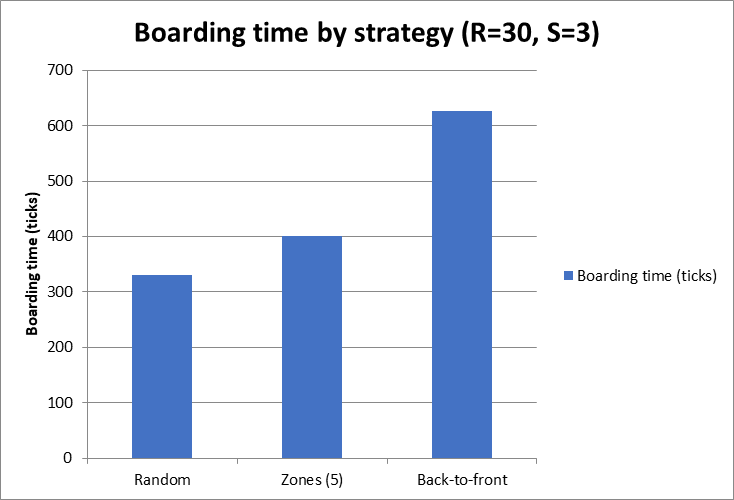
\includegraphics[width=0.88\linewidth,height=\textheight,keepaspectratio]{figures/fig1_strategy_time.png}

Figure 1. Boarding time by strategy (R=30, S=3): random fastest,
back-to-front slowest.

\subsection{3.2 Sensitivity analysis}\label{sensitivity-analysis}

\textbf{(a) Stow time (fixed \(R=30\)).}

{\def\LTcaptype{none} % do not increment counter
\begin{longtable}[]{@{}
  >{\raggedright\arraybackslash}p{(\linewidth - 10\tabcolsep) * \real{0.1667}}
  >{\raggedright\arraybackslash}p{(\linewidth - 10\tabcolsep) * \real{0.1667}}
  >{\raggedright\arraybackslash}p{(\linewidth - 10\tabcolsep) * \real{0.1667}}
  >{\raggedright\arraybackslash}p{(\linewidth - 10\tabcolsep) * \real{0.1667}}
  >{\raggedright\arraybackslash}p{(\linewidth - 10\tabcolsep) * \real{0.1667}}
  >{\raggedright\arraybackslash}p{(\linewidth - 10\tabcolsep) * \real{0.1667}}@{}}
\toprule\noalign{}
\begin{minipage}[b]{\linewidth}\raggedright
\(S\)
\end{minipage} & \begin{minipage}[b]{\linewidth}\raggedright
Random
\end{minipage} & \begin{minipage}[b]{\linewidth}\raggedright
Back-to-front
\end{minipage} & \begin{minipage}[b]{\linewidth}\raggedright
Zones (5)
\end{minipage} & \begin{minipage}[b]{\linewidth}\raggedright
Rel. random (back)
\end{minipage} & \begin{minipage}[b]{\linewidth}\raggedright
Rel. random (zones)
\end{minipage} \\
\midrule\noalign{}
\endhead
\bottomrule\noalign{}
\endlastfoot
1 & 239.1 & 325 & 250.0 & 1.36 & 1.05 \\
3 & 331.1 & 627 & 400.8 & 1.89 & 1.21 \\
6 & 472.2 & 1080 & 628.7 & 2.29 & 1.33 \\
\end{longtable}
}

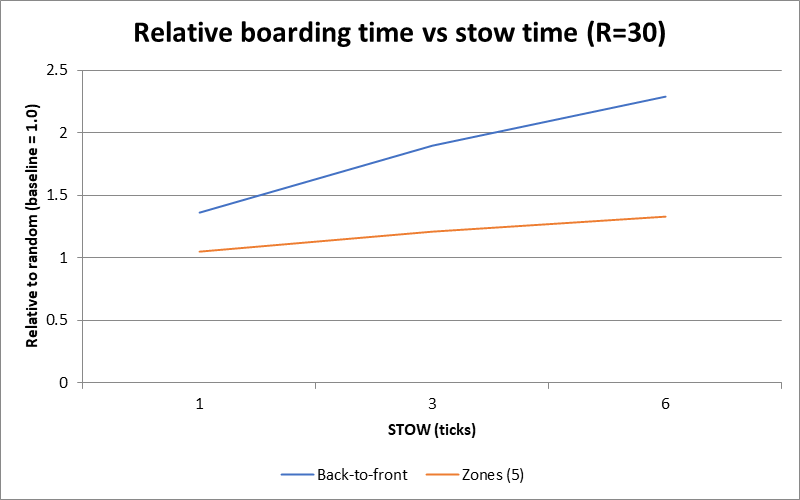
\includegraphics[width=0.88\linewidth,height=\textheight,keepaspectratio]{figures/fig2_relative_stow.png}

Figure 2. Relative boarding time vs stow time (R=30).

\textbf{(b) Number of rows (fixed \(S=3\)).}

{\def\LTcaptype{none} % do not increment counter
\begin{longtable}[]{@{}
  >{\raggedright\arraybackslash}p{(\linewidth - 10\tabcolsep) * \real{0.1667}}
  >{\raggedright\arraybackslash}p{(\linewidth - 10\tabcolsep) * \real{0.1667}}
  >{\raggedright\arraybackslash}p{(\linewidth - 10\tabcolsep) * \real{0.1667}}
  >{\raggedright\arraybackslash}p{(\linewidth - 10\tabcolsep) * \real{0.1667}}
  >{\raggedright\arraybackslash}p{(\linewidth - 10\tabcolsep) * \real{0.1667}}
  >{\raggedright\arraybackslash}p{(\linewidth - 10\tabcolsep) * \real{0.1667}}@{}}
\toprule\noalign{}
\begin{minipage}[b]{\linewidth}\raggedright
Rows \(R\)
\end{minipage} & \begin{minipage}[b]{\linewidth}\raggedright
Random
\end{minipage} & \begin{minipage}[b]{\linewidth}\raggedright
Back-to-front
\end{minipage} & \begin{minipage}[b]{\linewidth}\raggedright
Zones (5)
\end{minipage} & \begin{minipage}[b]{\linewidth}\raggedright
Rel. random (back)
\end{minipage} & \begin{minipage}[b]{\linewidth}\raggedright
Rel. random (zones)
\end{minipage} \\
\midrule\noalign{}
\endhead
\bottomrule\noalign{}
\endlastfoot
20 & 237.2 & 417 & 290.8 & 1.76 & 1.23 \\
30 & 331.1 & 627 & 400.8 & 1.89 & 1.21 \\
40 & 422.7 & 837 & 503.2 & 1.98 & 1.19 \\
\end{longtable}
}

\subsection{3.3 A faster strategy: strided descending
boarding}\label{a-faster-strategy-strided-descending-boarding}

We also tested strided orders: rows are split into groups by residue mod
6 --- group 1 = \{1, 7, 13, 19, 25\}, group 2 = \{2, 8, 14, 20, 26\},
and so on --- and each group is boarded either ascending or descending.
The \textbf{direction turns out to matter critically}: boarding each
group in descending order (\ldots, 19, 13, 7, 1) is far faster than
ascending order, and it even beats random boarding:

{\def\LTcaptype{none} % do not increment counter
\begin{longtable}[]{@{}llll@{}}
\toprule\noalign{}
Strategy & \(S=1\) & \(S=3\) & \(S=6\) \\
\midrule\noalign{}
\endhead
\bottomrule\noalign{}
\endlastfoot
Random & 239.1 & 331.1 & 472.2 \\
Zones (5) & 250.0 & 400.8 & 628.7 \\
Back-to-front & 325 & 627 & 1080 \\
Strided ascending (stride 6) & 322 & 562 & 922 \\
Strided descending (stride 6) & 214 & 286 & 394 \\
\end{longtable}
}

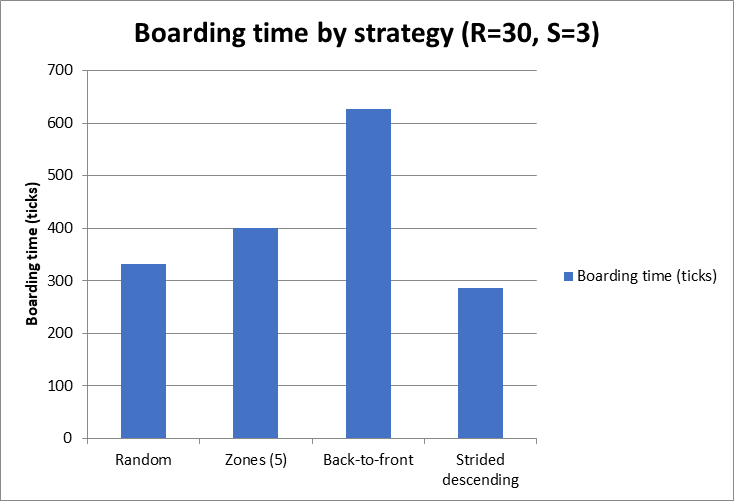
\includegraphics[width=0.88\linewidth,height=\textheight,keepaspectratio]{figures/fig3_including_strided.png}

Figure 3. Boarding time by strategy, including the strided-descending
order (R=30, S=3).

Strided descending boarding is the fastest --- e.g.~\textbf{286 vs 331}
(≈14\% faster) at \(S=3\) --- and the advantage grows with \(S\) (≈17\%
at \(S=6\)). The theory reproduces these values exactly (286/286).

\subsection{3.4 Why it is faster: parallelism and
blocking}\label{why-it-is-faster-parallelism-and-blocking}

To explain the differences above, the simulator records, at each tick
\(t\), two quantities: \(K(t)\) = the number of passengers
\textbf{stowing simultaneously} (parallelism), and \(B(t)\) = the number
of walkers \textbf{blocked} because the cell ahead is occupied. Over a
boarding of total length \(T\) ticks, we report the average parallelism
\((1/T)\sum_{t=1}^{T}K(t)\) and the total number of blocking events
\(\sum_{t=1}^{T}B(t)\).

{\def\LTcaptype{none} % do not increment counter
\begin{longtable}[]{@{}llll@{}}
\toprule\noalign{}
Strategy & Time (ticks) & Avg parallelism & Total blocking \\
\midrule\noalign{}
\endhead
\bottomrule\noalign{}
\endlastfoot
Strided descending & 286.0 & 1.26 & 1,305 \\
Random & 331.1 & 1.09 & 958 \\
Zones (5) & 400.8 & 0.90 & 2,989 \\
Back-to-front & 627.0 & 0.57 & 6,525 \\
\end{longtable}
}

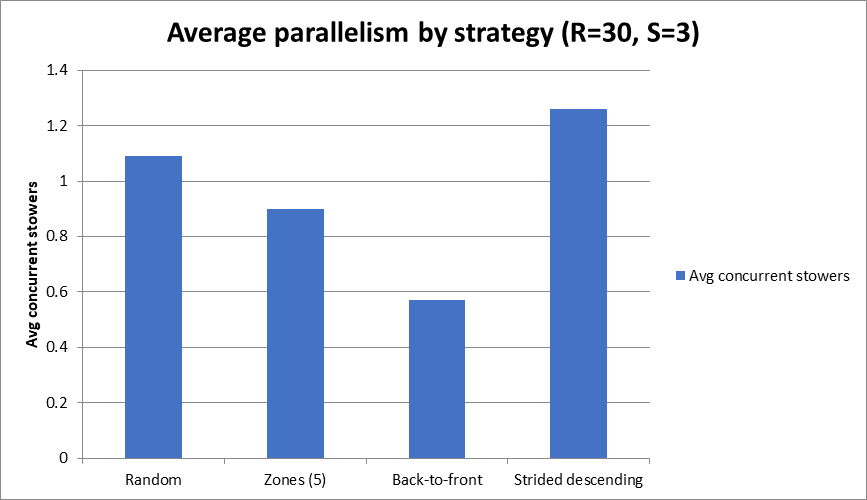
\includegraphics[width=0.88\linewidth,height=\textheight,keepaspectratio]{figures/fig4_parallelism.png}

Figure 4. Average parallelism by strategy (R=30, S=3).

Across all four strategies, higher parallelism goes with shorter
boarding time (Figure 4), and back-to-front combines the lowest
parallelism with the most blocking events. The theory of Section 2.3
explains this: in descending order each subsequent passenger stops
\emph{before} the previous stower's row, so nobody has to squeeze past
an occupied cell, whereas ascending order does the opposite and creates
cascading blocking.

\subsection{3.5 Effect of the stride}\label{effect-of-the-stride}

Direction is not the only design choice in strided boarding; the order
also depends on the stride \(k\) (rows are grouped by residue mod \(k\);
all earlier results use \(k=6\)). The stride acts through the same
mechanism as in Section 3.4: a larger \(k\) leaves fewer rows per group
and spreads stowing out (higher parallelism), whereas a smaller \(k\)
packs rows densely and invites cascading blocking. To see whether \(k\)
matters, we varied it for \(R=30\), \(S=3\):

{\def\LTcaptype{none} % do not increment counter
\begin{longtable}[]{@{}lll@{}}
\toprule\noalign{}
Stride \(k\) & Boarding time (ticks) & \\
\midrule\noalign{}
\endhead
\bottomrule\noalign{}
\endlastfoot
2 & 546 & \\
3 & 472 & \\
4 & 404 & \\
5 & 342 & \\
6 & 286 & \\
7 & 308 & \\
8 & 328 & \\
9 & 349 & \\
10 & 370 & \\
12 & 406 & \\
15 & 466 & \\
\end{longtable}
}

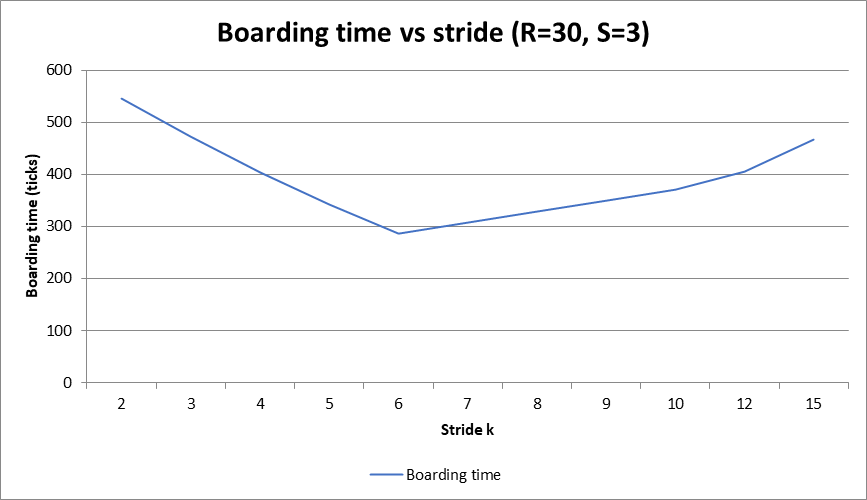
\includegraphics[width=0.88\linewidth,height=\textheight,keepaspectratio]{figures/fig5_stride.png}

Figure 5. Boarding time vs stride (R=30, S=3).

Boarding time is U-shaped in the stride --- lowest at \(k=6\) and rising
for both smaller and larger \(k\). A small stride packs closely spaced
rows into large groups (more interference within a group); a large
stride leaves too few rows per group (less parallelism). \(k=6\) splits
the cabin into blocks of \(R/k=5\) rows, balancing the two. This small,
self-contained optimum also foreshadows the open question in Section 5.

\section{4 Discussion}\label{discussion}

The strided-descending order is fastest, random already beats
back-to-front, and back-to-front is slowest. Random wins over
back-to-front because it spreads passengers across rows so several rows
stow simultaneously (highest parallelism, fewest blocking events);
back-to-front boards each row's six passengers consecutively so they
must stow one cell at a time (lowest parallelism, most blocking). The
sensitivity analysis (Figure 2) confirms that the gap grows with stow
time \(S\), exactly as the recurrence's \(+S\) blocking term predicts.

\section{5 Is there an optimal boarding order? (open
question)}\label{is-there-an-optimal-boarding-order-open-question}

The strided descending result shows that random is not necessarily
optimal. Two facts frame the search for an optimum:

\begin{itemize}
\tightlist
\item
  \textbf{Lower bounds.} \(T\ge\max\{N,\,3(R+1)+6S\}\). At \(R=30\),
  \(S=3\) this lower bound is \textbf{180}, while the best strategy
  found yields 286 --- so room remains.
\item
  \textbf{Mechanism.} Performance is governed by the longest chain of
  waits (the critical path). A good order keeps stowing spread over many
  rows and avoids forcing later passengers to pass an occupied cell.
\end{itemize}

We therefore \textbf{conjecture} that a near-optimal order is
``descending in spirit'': board so that passengers peel off toward the
front without ever passing a stower, while spreading stowing across as
many rows as possible. The true optimum likely lies between our strided
order and the lower bound. Finding (or proving) the globally optimal
order is an \textbf{open problem}; since the longest-path model
evaluates any order efficiently (\(O(N\cdot R)\) with preprocessing), it
can be used to search the space of orderings, and an analytical argument
may yield the optimum directly. We leave this to future work.

\section{6 Limitations and Future
Work}\label{limitations-and-future-work}

\begin{itemize}
\tightlist
\item
  Simplified model: no assigned-seat interference, no dual aisle or
  second door.
\item
  The theoretical recurrence uses a naive \(O(N)\) search for \(j\); it
  can be reduced to \(O(N\cdot R)\) overall with preprocessing.
\item
  Future work: add the ``Steffen method'' and window--middle--aisle
  boarding; test a model in which parallelism is disabled as a direct
  causal test.
\end{itemize}

\section{7 Conclusion}\label{conclusion}

In this simulation the strided-descending order is fastest, random beats
back-to-front, and back-to-front is slowest. The differences are
explained by a measured mechanism (parallelism and blocking) and by an
exact longest-path (max-plus) model that reproduces the simulation
bit-for-bit. Boarding so that passengers stop before the previous stower
keeps the critical path short --- the underlying principle behind the
observed gaps.

\section{Data and Code Availability}\label{data-and-code-availability}

The simulation, the longest-path (max-plus) model, the interactive
visualizer, and this report are openly available at
\url{https://github.com/Huang-1226/boarding-order-simulation} and
archived with a DOI: \url{https://doi.org/10.5281/zenodo.23186759}. The
text preparation and code implementation were assisted by the AI
assistant opencode (see the Report on Use of AI Tools at the end of this
document).

\section{References}\label{references}

\begin{enumerate}
\def\labelenumi{\arabic{enumi}.}
\tightlist
\item
  Baccelli, F., Cohen, G., Olsder, G. J., \& Quadrat, J.-P. (1992).
  \emph{Synchronization and Linearity: An Algebra for Discrete Event
  Systems}. Wiley.
\item
  Bachmat, E., Berend, D., Sapir, L., Skiena, S., \& Stolyarov, N.
  (2009). Analysis of airplane boarding times. \emph{Operations
  Research}, 57(2), 499--513.
\item
  Steffen, J. H. (2008). Optimal boarding method for airline passengers.
  \emph{Journal of Air Transport Management}, 14(3), 146--150.
\item
  Van Landeghem, H., \& Beuselinck, A. (2002). Reducing passenger
  boarding time in airplanes: a simulation-based approach.
  \emph{European Journal of Operational Research}, 142(2), 294--308.
\item
  opencode (AI coding assistant), deepseek-v4.1-flash model, October
  2026. Used for code implementation and report text preparation; see
  Report on Use of AI Tools.
\end{enumerate}

\section{Report on Use of AI Tools}\label{report-on-use-of-ai-tools}

The author used AI tools as follows. All scientific content --- the
simulation, the longest-path (max-plus) model, the data analysis, and
the conclusions --- is the author's own; every AI-generated or
AI-rewritten item was reviewed and corrected by the author, who takes
full responsibility.

\begin{enumerate}
\def\labelenumi{\arabic{enumi}.}
\tightlist
\item
  \textbf{opencode} (AI coding assistant), deepseek-v4.1-flash model
  (October 2026 version). Under the author's direction, it implemented
  the models in Python and JavaScript, built the interactive simulation
  website and UI, and assisted with the report's language polishing,
  structural editing, and Chinese--English translation.
\item
  The author was responsible for the research topic, the study design,
  and the model design.
\end{enumerate}

\textbf{Statement:} All AI output was checked and corrected item by
item; this disclosure is for transparency and does not imply that AI
contributed to the scientific conclusions.

\end{document}
